\section{Repeater and Communication Basics}
\label{section:repeater_basics}

\subsection*{Understanding Repeaters}

A repeater is an automated station that extends the range of communications by receiving signals on one frequency (the input frequency) and simultaneously retransmitting them on another frequency (the output frequency). This system allows operators to communicate over much greater distances than would be possible with direct communication, particularly useful in areas with challenging terrain.


Repeaters are typically:
\begin{itemize}
    \item Located in elevated positions (hills, towers, tall buildings)
    \item Equipped with better antennas and more powerful transmitters than typical portable or mobile stations
    \item Designed to operate automatically without an operator present
    \item Used to greatly extend the communication range of lower-powered stations
\end{itemize}

Key repeater concepts include:
\begin{itemize}
    \item \textbf{Offset}: The difference between input and output frequencies (e.g., ±600 kHz for 2 meters, ±5 MHz for 70 cm)
    \item \textbf{Access Tones}: Special sub-audible tones (CTCSS) or digital codes that may be required to activate the repeater
    \item \textbf{Coverage Area}: The geographical area where the repeater can be effectively used
    \item \textbf{Timeout Timer}: A safety feature that limits the length of transmissions
\end{itemize}

\begin{wrapfigure}{r}{0.4\textwidth}
    \centering
    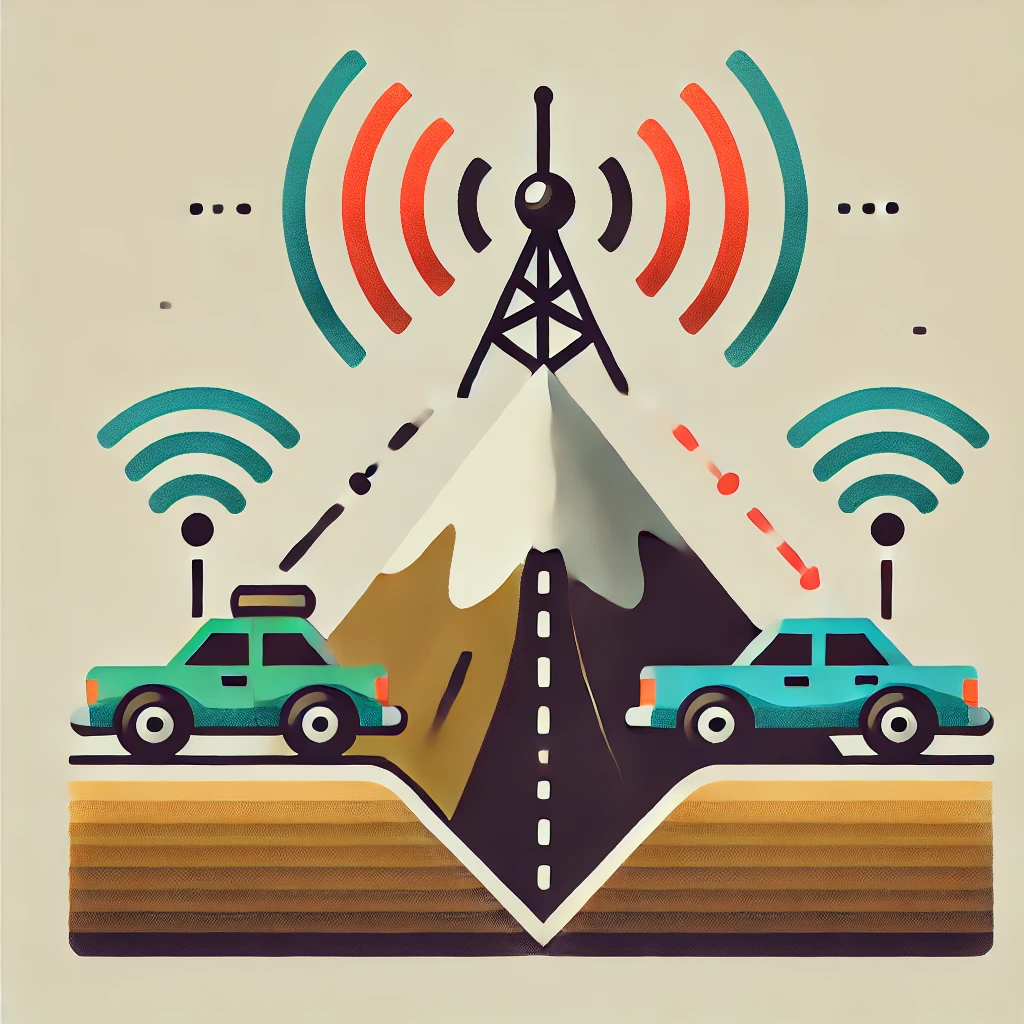
\includegraphics[width=0.35\textwidth]{tech/organized/chapter_2/images/repeater.png}
    \caption{How two stations can communicate over greater distances through a repeater. }
    \label{fig:repeater_operation}
\end{wrapfigure}

For example, if a mobile station can normally communicate directly (simplex) for 5-10 miles, using a repeater might extend this range to 50 miles or more, depending on terrain and repeater location.

\subsection*{Repeater Frequency Offsets}
The difference between a repeater's transmit and receive frequencies (offset) is crucial because it allows the repeater to receive and transmit simultaneously without interference. Standard offsets vary by band:
\begin{itemize}
    \item 2 meter band: ±600 kHz offset
    \item 70 cm band: ±5 MHz offset
\end{itemize}

\subsection*{National Calling Frequency for FM Simplex Operations}
In the 2 meter band, the national calling frequency for FM simplex operations is 146.520 MHz. This frequency is designated as a common channel where operators can initiate contact with other stations. The importance of this frequency lies in its universal recognition among amateur radio operators. When an operator calls on 146.520 MHz, they are essentially broadcasting a signal to any station within range, inviting a response.

\subsection*{Procedural Signal 'CQ'}
The procedural signal 'CQ' is used in amateur radio to indicate a general call to any station. When an operator transmits 'CQ', they are essentially saying, "I am calling any station that can hear me." This signal is particularly useful when an operator is looking to make contact with any available station, rather than a specific one. The term 'CQ' has its origins in maritime communication, where it was used as a general call to all ships.

\subsection*{Repeater Offset}
The term 'repeater offset' refers to the difference between a repeater's transmit and receive frequencies. This offset is necessary to prevent the repeater from interfering with its own transmissions. For example:

\begin{itemize}
    \item If a 2-meter repeater receives on 147.000 MHz, it might transmit on 147.600 MHz (a +600 kHz offset)
    \item If a 70cm repeater receives on 446.000 MHz, it might transmit on 441.000 MHz (a -5 MHz offset)
\end{itemize}

\begin{table}[h!]
    \centering
    \begin{tabular}{|l|l|l|l|}
        \hline
        \textbf{Band} & \textbf{Frequency Range} & \textbf{Common Offset} & \textbf{Direction} \\
        \hline
        2 meters & 144-148 MHz & 600 kHz & + above 147 MHz \\
        & & & - below 147 MHz \\
        \hline
        70 cm & 440-450 MHz & 5 MHz & - typical in USA \\
        & & & + in some regions \\
        \hline
    \end{tabular}
    \caption{Standard Repeater Frequency Offsets}
    \label{tab:repeater_offsets}
\end{table}

The offset direction (positive or negative) is standardized by band and region. For the 2-meter band in the United States, the offset direction changes at 147 MHz - negative below and positive above. This standardization helps operators quickly determine the correct transmit frequency when using a repeater.

\subsection*{Questions}

\begin{tcolorbox}[colback=gray!10!white,colframe=black!75!black,title={T2A01}]
What is a common repeater frequency offset in the 2 meter band?
\begin{enumerate}[label=\Alph*),noitemsep]
    \item Plus or minus 5 MHz
    \item \textbf{Plus or minus 600 kHz}
    \item Plus or minus 500 kHz
    \item Plus or minus 1 MHz
\end{enumerate}
\end{tcolorbox}
A common repeater frequency offset in the 2 meter band is $\pm 600$ kHz. This offset is widely used to ensure that the repeater can transmit and receive simultaneously without interference. The other options are not standard offsets for the 2 meter band.
%memory_trick T2A01

\begin{tcolorbox}[colback=gray!10!white,colframe=black!75!black,title={T2A02}]
What is the national calling frequency for FM simplex operations in the 2 meter band?
\begin{enumerate}[label=\Alph*),noitemsep]
    \item \textbf{146.520 MHz}
    \item 145.000 MHz
    \item 432.100 MHz
    \item 446.000 MHz
\end{enumerate}
\end{tcolorbox}
The national calling frequency for FM simplex operations in the 2 meter band is 146.520 MHz. This frequency is universally recognized and used by amateur radio operators to initiate contact with other stations. The other frequencies listed are not designated as national calling frequencies.
%memory_trick T2A02

\begin{tcolorbox}[colback=gray!10!white,colframe=black!75!black,title={T2A03}]
What is a common repeater frequency offset in the 70 cm band?
\begin{enumerate}[label=\Alph*),noitemsep]
    \item \textbf{Plus or minus 5 MHz}
    \item Plus or minus 600 kHz
    \item Plus or minus 500 kHz
    \item Plus or minus 1 MHz
\end{enumerate}
\end{tcolorbox}
A common repeater frequency offset in the 70 cm band is $\pm 5$ MHz. This offset is necessary to prevent interference between the repeater's transmit and receive frequencies. The other options are not standard offsets for the 70 cm band.
%memory_trick T2A03

\begin{tcolorbox}[colback=gray!10!white,colframe=black!75!black,title={T2A04}]
What is an appropriate way to call another station on a repeater if you know the other station's call sign?
\begin{enumerate}[label=\Alph*),noitemsep]
    \item Say "break, break," then say the station's call sign
    \item \textbf{Say the station's call sign, then identify with your call sign}
    \item Say "CQ" three times, then the other station's call sign
    \item Wait for the station to call CQ, then answer
\end{enumerate}
\end{tcolorbox}
The appropriate way to call another station on a repeater is to say the station's call sign, followed by your own call sign. This method ensures that the other station knows who is calling and who is responding. The other options are either incorrect or not standard procedures.
%memory_trick T2A04

\begin{tcolorbox}[colback=gray!10!white,colframe=black!75!black,title={T2A05}]
How should you respond to a station calling CQ?
\begin{enumerate}[label=\Alph*),noitemsep]
    \item Transmit "CQ" followed by the other station’s call sign
    \item Transmit your call sign followed by the other station’s call sign
    \item \textbf{Transmit the other station’s call sign followed by your call sign}
    \item Transmit a signal report followed by your call sign
\end{enumerate}
\end{tcolorbox}
When responding to a station calling CQ, you should transmit the other station’s call sign followed by your own call sign. This method ensures that the other station knows who is responding to their call. The other options are either incorrect or not standard procedures.
%memory_trick T2A05

\begin{tcolorbox}[colback=gray!10!white,colframe=black!75!black,title={T2A06}]
Which of the following is required when making on-the-air test transmissions?
\begin{enumerate}[label=\Alph*),noitemsep]
    \item \textbf{Identify the transmitting station}
    \item Conduct tests only between 10 p.m. and 6 a.m. local time
    \item Notify the FCC of the transmissions
    \item All these choices are correct
\end{enumerate}
\end{tcolorbox}
When making on-the-air test transmissions, it is required to identify the transmitting station. This is a fundamental rule in amateur radio operations to ensure that all transmissions are properly identified. The other options are either incorrect or not required for test transmissions.
%memory_trick T2A06

\begin{tcolorbox}[colback=gray!10!white,colframe=black!75!black,title={T2A07}]
What is meant by "repeater offset"?
\begin{enumerate}[label=\Alph*),noitemsep]
    \item \textbf{The difference between a repeater’s transmit and receive frequencies}
    \item The repeater has a time delay to prevent interference
    \item The repeater station identification is done on a separate frequency
    \item The number of simultaneous transmit frequencies used by a repeater
\end{enumerate}
\end{tcolorbox}
The term "repeater offset" refers to the difference between a repeater’s transmit and receive frequencies. This offset is necessary to prevent the repeater from interfering with its own transmissions. The other options do not accurately describe the concept of repeater offset.
%memory_trick T2A07

\begin{tcolorbox}[colback=gray!10!white,colframe=black!75!black,title={T2A08}]
What is the meaning of the procedural signal "CQ"?
\begin{enumerate}[label=\Alph*),noitemsep]
    \item Call on the quarter hour
    \item Test transmission, no reply expected
    \item Only the called station should transmit
    \item \textbf{Calling any station}
\end{enumerate}
\end{tcolorbox}
The procedural signal "CQ" means "calling any station." It is used to initiate contact with any station that can hear the transmission. The other options do not accurately describe the meaning of "CQ."
%memory_trick T2A08

\subsection*{Summary}
This section covered several key concepts related to repeater and communication basics in amateur radio:
\begin{itemize}
    \item \textbf{Repeater frequency offsets}: The difference between a repeater's transmit and receive frequencies, which is essential for preventing interference and extending communication range.
    \item \textbf{Simplex operations}: Direct communication between two stations without the use of a repeater, with the national calling frequency for FM simplex operations in the 2 meter band being 146.520 MHz.
    \item \textbf{Calling procedures}: The correct way to call another station on a repeater and how to respond to a station calling CQ.
    \item \textbf{Repeater terminology}: Understanding terms like "repeater offset" and the procedural signal "CQ" is crucial for effective communication in amateur radio.
\end{itemize}


